\documentclass[11pt]{article}
\usepackage[T1]{fontenc}
\usepackage{lmodern}
\usepackage[margin=1in,letterpaper]{geometry}
\usepackage{amsmath,amssymb,booktabs,array,xcolor}
\usepackage{textcomp}
\usepackage[hidelinks]{hyperref}
\usepackage{graphicx}
\graphicspath{{paper_figures/}{./}{../paper_figures/}}
\usepackage{tabularx}
\usepackage{caption}
\captionsetup{font=small,labelfont=bf,skip=4pt}
\usepackage{placeins}
\usepackage{float}
\usepackage{seqsplit}
\renewcommand{\topfraction}{0.9}
\renewcommand{\bottomfraction}{0.85}
\renewcommand{\textfraction}{0.07}
\renewcommand{\floatpagefraction}{0.75}
\setcounter{topnumber}{4}
\setcounter{bottomnumber}{4}
\setcounter{totalnumber}{8}
\emergencystretch=2.5em

\newcommand{\eebar}{\bar{e}_{31}}
\newcommand{\Xibar}{\bar{\Xi}_{33}}
\newcommand{\cbar}{\bar{c}_{11}^{E}}
\newcommand{\fn}[1]{\texttt{\seqsplit{#1}}}

\title{\bfseries Exact Radial-Determinant Flexural Frequencies of a
Monolithic Thickness-Poled Piezoelectric Ring: An Open-Circuit-Equals-Short-Circuit Theorem and a Segmented-Electrode Sensing Admittance}
\author{Garrek McCune$^{a,*}$, Daniel Stutts$^{a}$\\
\small\itshape $^a$Mechanical and Aerospace Engineering,\\
Missouri University of Science and Technology, Rolla, MO 65409, USA\\
\small\upshape $^*$Corresponding author. E-mail: ghmkfh@umsystem.edu}
\date{DRAFT --- \today}
% Supplementary Material mapping (PAPER5_MONOLITHIC_PIEZO_SUPPLEMENTARY.tex):
%   S.1  cubic consistency condition and the OC=SC theorem, in full
%   S.2  elastic-limit gate against the closed-ring solver
%   S.3  finite-element cross-check, provenance and discriminator
%   S.4  e31 inverse: gates, sensitivity, reflection twin
%   S.5  overtones and thickness sweep, full numeric tables
%   S.6  mixed-edge (C-F/F-C) bit-identical reduction proof
%   S.7  force-driven sensing admittance: 12x12 construction and gates
%   S.8  cluster job provenance
% Main text contains no job numbers.

\begin{document}
\maketitle

\begin{abstract}
A homogeneous, thickness-poled piezoceramic annulus -- one ceramic
spanning the full plate thickness, electroded only on its two faces, with
no elastic host -- is solved by the same exact radial-determinant method
used for a layered piezoelectric sandwich, but with a different
through-thickness potential. Two results follow from removing the offset
skins. First, because a spatially uniform electrode voltage produces a
field symmetric about this plate's own neutral surface, its piezoelectric
moment integrates to zero for every mechanical boundary condition tested:
fully electroded open-circuit flexure coincides exactly with short-circuit
flexure, and the electrode-voltage admittance degenerates to a
frequency-independent capacitor, $Y=j\omega C_0$ with
$k_{\mathrm{eff}}^2\equiv0$. Second, the short-circuit frequency itself
becomes the identifying piezoelectric signal, sitting $+1.94\%$
(free--free) to $+1.44\%$ (free--clamped) above the same plate's purely
elastic frequency on a representative PZT-4 geometry -- an order of
magnitude larger than the corresponding split on a steel-dominated
layered sandwich, and well conditioned for inverting the piezoelectric
stress constant $e_{31}$: a $0.01\%$ frequency uncertainty propagates to
only $0.32\%$--$0.34\%$ of $e_{31}$. The through-thickness potential is
closed by a Galerkin projection of the electric enthalpy, which makes the
long-wave short-circuit stiffening exact; the thickness-integrated Gauss
law used for layered plates overstates it by $12/\pi^2$. The elastic
limit agrees with an independent closed-ring solver to
$4.8\times10^{-10}$ relative, and finite elements confirm both the
coincidence and the stiffening magnitude, reproducing the closed-form
split to $0.1\%$ of its value. Because the voltage-driven route
is trivial, sensing instead reads the mechanical side of the same
coupling: a harmonic radial force drives a genuinely resonant charge
response on a segmented electrode, even though the same force drives an
identically zero charge on the full electroded face. A symmetric,
thickness-poled monolithic plate can therefore be neither voltage-actuated
nor full-electrode-sensed in flexure, but can be force-driven and
segment-sensed -- the textbook justification for unimorph and bimorph
bending actuators, derived here as an exact, closed-form property of the
radial-determinant operator.
\end{abstract}

\noindent\textbf{Keywords:} piezoelectric annular plate; monolithic
piezoceramic; open-circuit; short-circuit; electromechanical coupling;
radial determinant; free--free flexure; sensing admittance.

\section{Introduction}\label{sec:intro}
A companion paper from this group solved a layered annular plate --
an isotropic host with identical thickness-polarized piezoceramic skins
bonded to both faces -- by an exact radial-determinant method, and used
the resulting open-circuit flexural frequency to invert the piezoelectric
stress constant $e_{31}$ at a precision the corresponding short-circuit
frequency could not reach \cite{mccune2026piezo}. That construction is a
deliberate choice of specimen: a thin piezoceramic layer offset from the
plate's neutral axis, so that even a spatially uniform electrode voltage
produces a bending moment. It is not, however, the specimen most readily
available for a physical test. A commercial thickness-poled piezoceramic
ring -- the kind sold as a ultrasonic transducer element or a buzzer disk
-- is not a host with bonded skins; it is one ceramic, poled through its
full thickness, electroded on its two faces. The present paper asks the
same questions of that geometry.

The answers are qualitatively different, not merely quantitatively so.
On the layered plate, the piezoceramic skins sit at $\lvert z\rvert>h$,
offset from the neutral surface, so a spatially uniform through-thickness
field has a nonzero moment arm and free--free open-circuit flexure
genuinely splits from short-circuit flexure. On the homogeneous
monolithic plate the ceramic \emph{is} the neutral surface: a spatially
uniform field is symmetric about it, and the piezoelectric moment it
would produce integrates to zero over $\lvert z\rvert\le H$ for every
mechanical boundary condition, not only the clamped--clamped case where
the layered plate's own coincidence already held. That is the textbook
reason real bending-mode piezoelectric actuators are built as unimorphs
or bimorphs and never as symmetric monolithic slabs: this paper derives
that fact as a closed-form theorem for the exact radial-determinant
operator, rather than assuming it, and then asks what \emph{is}
identifiable and sensible on the specimen that is actually a single
poled ceramic.

Two results follow directly from removing the offset skins. First, the
short-circuit flexural frequency itself -- not an open-circuit split --
becomes the piezoelectric signal, because the whole plate thickness is
now piezoceramic rather than a thin fraction of it: the short-circuit
coupling on this stacking is a few percent in frequency, where it was two
to three orders of magnitude smaller on the layered plate. Second,
because the voltage-driven admittance degenerates to a frequency-%
independent capacitor, the free--free resonance/antiresonance
identification used on the layered plate is not available here. Sensing
instead uses the mechanical side of the same electromechanical coupling:
a harmonic radial force on the plate drives a genuinely resonant charge
response, provided the sensing electrode is a proper subset of the
grounded face rather than the whole face -- the full-face charge is
itself identically zero, by the same cancellation that kills the
voltage-driven admittance, read from the other electrical port.

Parashar gave a Rayleigh--Ritz treatment, with experiment, of a
radially poled annular piezoceramic actuator whose flexural actuation
mechanism is shear-induced ($d_{15}$) rather than thickness-poled
bending, on Mindlin rather than Kirchhoff kinematics \cite{parashar2013}.
That is a different poling direction, a different actuation mechanism,
and a different plate theory; the coincidence theorem of this paper does
not apply to it, and it is not scored here. It is a natural second phase
on the same family of exact radial-determinant methods and is left for
later work. Holland's contour-mode analysis of an unpoled elastic disk
\cite{holland1966} is the classical reference for the in-plane
(extensional, $k_p$) response the same physical ring would show on its
impedance spectrum; that response is disclosed here as a boundary of
scope, not built.

The underlying elastic operator, and the exact radial-determinant method
itself, are the closed-annulus reduction used throughout this project's
series \cite{mccune2026ring}: integer circumferential order $n$, a
boundary-condition-selected radial edge matrix, and frequencies as zeros
of that determinant. The layered-plate piezoelectric extension
\cite{mccune2026piezo} added a through-thickness potential that vanishes
on every electrode, after Duan, Quek and Wang \cite{duan2005}, and the
constitutive reduction of Liu, Wang and Quek \cite{liu2002}; the present
paper reuses that constitutive reduction on a single ceramic spanning the
full thickness, with a potential shape that is even, not odd, about the
plate's own midplane, which is the root cause of every difference from
the layered result. Both papers close the electrical equation by the
same Galerkin projection of the electric enthalpy that produces the
mechanical one, rather than by Duan, Quek and Wang's thickness-integrated
Gauss law; \S\ref{sec:sc} explains why that choice changes the
short-circuit stiffening by a fixed factor.

What is not claimed: in-plane (extensional, contour-mode) piezoelectric
coupling as a headline result, though a negative control confirming that
a uniform voltage \emph{does} couple to membrane force is included; a
radially poled or shear-actuated ($d_{15}$) specimen; a laboratory
specimen; or a joint fit of elastic stiffness and $e_{31}$ from a single
frequency.

\section{Theory}\label{sec:theory}

\subsection{Kinematics and constitutive reduction}\label{sec:kinematics}
The ring occupies $r_i\le r\le r_o$, $\lvert z\rvert\le H$ (full thickness
$2H$), one homogeneous piezoceramic, thickness-polarized, electroded only
on the two faces $z=\pm H$. There is no elastic host and no electrode at
the midplane. Kirchhoff kinematics are unchanged from the elastic and
layered-piezoelectric cases,
\begin{equation}
u_r=-z\,\partial_r w,\qquad
u_\theta=-z\,r^{-1}\partial_\theta w,\qquad
u_z=w(r,\theta,t),
\end{equation}
giving strains odd in $z$ and $\varepsilon_{rr}+\varepsilon_{\theta\theta}
=-z\nabla^2 w$. Transverse shear vanishes identically, so $e_{15}$ never
enters, as in the layered case.

Plane-stress reduction of the full three-dimensional piezoceramic
constants follows the same construction as the layered plate
\cite{liu2002,mccune2026piezo}:
\begin{equation}
\cbar=c_{11}^E-\frac{(c_{13}^E)^2}{c_{33}^E},\qquad
\eebar=e_{31}-\frac{c_{13}^E}{c_{33}^E}e_{33},\qquad
\Xibar=\Xi_{33}+\frac{e_{33}^2}{c_{33}^E}.
\label{eq:reduced}
\end{equation}
At the material point used throughout this paper (\S\ref{sec:forward}),
$\eebar\approx-4.85\,\mathrm{C\,m^{-2}}$: the sign of the reduced constant
is opposite the tabulated $e_{31}$, the same reduction and the same sign
flip as the layered plate. Bending stiffness has no separate host or
layer terms; the whole thickness is piezoceramic,
\begin{equation}
d=\tfrac{2}{3}\cbar H^3,\qquad
\nu_p=\bar c_{12}^E/\cbar,\qquad
A_1=\tfrac12(1-\nu_p)d,\qquad
A_2=2\rho H.
\label{eq:d}
\end{equation}
The piezoelectric extra stress in $\sigma_{rr}$ and $\sigma_{\theta\theta}$
is $-\eebar E_z$. Its contribution to the membrane resultant
$N_{rr}=\int_{-H}^{H}\sigma_{rr}\,\mathrm dz$ and to the bending resultant
$M_{rr}=\int_{-H}^{H}z\,\sigma_{rr}\,\mathrm dz$ splits on the parity of
$E_z$ about the plate midplane: an $E_z$ that is even in $z$ (a spatially
constant field, produced by a uniform electrode voltage) contributes to
$N_{rr}$ and integrates to exactly zero in $M_{rr}$, because $z$ is odd
and the interval $[-H,H]$ is symmetric; an $E_z$ that is odd in $z$ does
the reverse. On the layered plate the piezoceramic sits entirely at
$\lvert z\rvert>h$, so even a spatially constant field has a nonzero
moment arm about the neutral axis and produces a genuine bending moment.
On this monolithic plate the ceramic occupies the neutral surface itself,
so the even/constant field is symmetric about it and contributes no
moment at all, for any thickness or any material constants. That single
parity fact is the source of every result in this paper: a spatially
uniform face voltage is, on this stacking, an extensional actuator and
not a flexural one.

\subsection{Short-circuit potential and the closing cubic}
\label{sec:sc}
With both faces grounded, $\phi(\pm H)=0$, the potential ansatz is an
even quadratic that vanishes at both faces,
\begin{equation}
\phi(r,\theta,z,t)=\bar\phi(r,\theta,t)\Bigl(1-\frac{z^2}{H^2}\Bigr).
\label{eq:phi-sc}
\end{equation}
$\phi$ is even in $z$; the interior field $E_z=2z\bar\phi/H^2$ is odd,
and is therefore the flexural actuator identified in
\S\ref{sec:kinematics}. The equation for $\bar\phi$ comes from the same
projection as the flexural equation: stationarity of the
thickness-integrated electric enthalpy with respect to $\bar\phi$, with
the ansatz itself as the weight. The alternative used for layered plates
by Duan, Quek and Wang \cite{duan2005} closes the electrical equation by
integrating Gauss's law through the thickness, i.e.\ with a unit weight,
while the coupling reaches the flexural equation through the moment,
i.e.\ with weight $z$. The two projections are then not conjugate, and
the long-wave short-circuit stiffening depends on which is used. With a
sinusoidal profile, $\bar\phi\cos(\pi z/2H)$, the Gauss-law closure
overstates the exact long-wave increment by exactly $12/\pi^2=1.216$,
and the same-weight projection understates it by $96/\pi^4=0.986$
(Supplementary~\S~S.1). The quadratic \eqref{eq:phi-sc} is the unique
one-term profile for which the same-weight projection is exact in the
long-wave limit: it reproduces the thin-plate short-circuit result
obtained directly from $\partial_zD_z=0$ with $\phi(\pm H)=0$, which is
$\eebar^{\,2}/\Xibar$ added to both $\cbar$ and $\bar c_{12}^E$.
Substituting into the moment/shear resultants and the projected
electrical equation, and positing
$\bar\phi=\chi\bar w$ with $\chi$ independent of $r$, again produces two
Helmholtz equations for $\bar w$ that are simultaneously satisfiable only
when $\chi$ and the radial eigenvalue $\lambda$ satisfy a cubic
consistency condition in $\chi$ (Supplementary~\S~S.1); the coefficients
of that cubic are not obtained by substituting the layered plate's own
layer thickness $h_1\to2H$ into its cubic, because the two potential
shapes have different parity about the plate midplane. The cubic has
three roots $(\chi_i,\lambda_i)$, each a function of the trial frequency
$\omega$; for each root the radial problem is second-order Helmholtz,
with Bessel pair $(J_n,Y_n)$ or modified pair $(I_n,K_n)$ by the sign of
$\lambda_i$. Three branches times two radial functions is a
six-dimensional basis, matching the sixth-order coupled system, exactly
as on the layered plate. Setting $\eebar\to0$ is again a singular limit
of the cubic, so the purely elastic ring is assembled as a separate
two-branch $4\times4$, gated independently in \S\ref{sec:elastic}.

Edge conditions are mechanical plus the insulated-rim electrical
condition $\partial\bar\phi/\partial r=0$ at $r_i$ and $r_o$. Four
mechanical edge pairings are used in this paper, in Paper~3's
inner-then-outer naming \cite{mccune2026ring}: free--free
($M_{rr}=Q_r^{\mathrm{eff}}=0$ at both edges, with
$Q_r^{\mathrm{eff}}=Q_r+r^{-1}\partial M_{r\theta}/\partial\theta$ the Kirchhoff
effective shear), clamped--clamped ($w=w'=0$ at both
edges), clamped--free (inner clamped, outer free), and free--clamped (the
swap). Each pairing selects the corresponding rows of the $6\times6$
short-circuit determinant, with the two insulated-rim rows unchanged, and
the free--free and clamped--clamped determinants are literal special
cases of the same mixed-edge row-selection logic used for the
clamped--free and free--clamped pairs (Supplementary~\S~S.6). Zeros are
found by a real-part sign-flip bisection on a pre-registered frequency
bracket, with a hi-side-only negative-control bracket that is not
permitted to flip; published values, where any exist, are never used to
seed a search.

\subsection{Open-circuit flexure coincides with short-circuit flexure}
\label{sec:oc}
Open-circuit replaces the grounded faces with a single floating bus at
unknown voltage $V(t)$, with total electrode charge constrained to zero.
The leading through-thickness potential is the linear particular
solution plus the same interior profile,
\begin{equation}
\phi=\frac{V(t)\,z}{2H}+\bar\phi(r,\theta,t)\Bigl(1-\frac{z^2}{H^2}\Bigr).
\label{eq:phi-oc}
\end{equation}
The linear term's field $E_z^{\mathrm{lin}}=-V/(2H)$ is spatially
constant -- even in $z$ -- so, by \S\ref{sec:kinematics}, it contributes
identically zero to $M_{rr}$ for any $V$, any geometry, any material
constants. It also does not enter $Q_r^{\mathrm{eff}}$ or the interior field equations:
the bus is a single equipotential surface with no $r,\theta$ structure,
so its field has zero radial gradient, and its cross term with the
interior profile integrates to zero through the thickness
($\int_{-H}^{H}\partial_z(1-z^2/H^2)\,\mathrm dz=0$). The projected
electrical equation and the flexural motion equation are therefore
exactly the short-circuit pair, driven by $\bar\phi$ alone. The unknown
bus voltage $V$ is not a second frequency-domain unknown; it is fixed
\emph{after} the mode is known, by the single scalar constraint $Q=0$.
The bus charge conjugate to $V$ in the same enthalpy has no motional
part at all -- the linear field's strain coupling carries the odd
weight $\int_{-H}^{H}z\,\mathrm dz=0$ and its cross term with
$\bar\phi$ vanishes as above -- so
\begin{equation}
Q=-C_0V,\qquad
C_0=\frac{\Xibar A}{2H},\qquad A=\pi(r_o^2-r_i^2),
\label{eq:Vsensor}
\end{equation}
and $Q=0$ gives $V=0$: a flexural mode develops no voltage on an
open-circuit full-face bus.
\textbf{Theorem.} For a homogeneous, thickness-polarized, fully
electroded Kirchhoff annulus under this ansatz, open-circuit flexural
frequencies coincide with short-circuit flexural frequencies exactly, for
every mechanical boundary condition. The IEEE electromechanical coupling
factor $k_{\mathrm{eff}}^2=1-(f_r/f_a)^2$ built from flexural resonance
and antiresonance is identically zero. A spatially uniform electrode
voltage cannot actuate flexure on this specimen.

This is the reverse of the layered plate's own result. There, offset
skins give a spatially constant field a nonzero moment arm, so
free--free open-circuit genuinely splits from short-circuit and only the
clamped--clamped pairing coincides, because Green's identity forces the
electrode-charge term that carries $V$ to vanish when the edge rotation
is zero everywhere \cite{mccune2026piezo}. Here the coincidence holds
regardless of the mechanical edge, because $V$ never enters the moment
balance at all -- the geometric offset that made the layered plate's
coincidence a special case of one boundary condition does not exist on a
symmetric monolithic plate. Do not invert an open-circuit-versus-%
short-circuit split for $e_{31}$ on this stacking, and do not add a
frequency solver expecting one; by \eqref{eq:Vsensor} the full-face
electrode does not even sense the flexural mode, which is why
\S\ref{sec:Y-sense} partitions it.

\subsection{Elastic limit}\label{sec:elastic}
Setting $\eebar=0$ (and $\bar\phi=0$) recovers an isotropic Kirchhoff
ring of thickness $2H$ with bending stiffness $D=d$ of
\eqref{eq:d} and Poisson ratio $\nu=\nu_p$. Matching the standard
isotropic-plate stiffness $D=Eh^3/[12(1-\nu^2)]$ at $h=2H$ requires
\begin{equation}
E=\cbar\bigl(1-\nu_p^2\bigr)=\frac{(\cbar)^2-(\bar c_{12}^E)^2}{\cbar},
\qquad \nu=\nu_p=\bar c_{12}^E/\cbar.
\label{eq:Enu}
\end{equation}
This is the first numerical gate applied in \S\ref{sec:forward}, before
any coupled number is trusted: the purely elastic $4\times4$ at
$(E,\nu,\rho,h=2H)$ from \eqref{eq:Enu} must agree with an independently
implemented closed-annulus Kirchhoff solver \cite{mccune2026ring} that
shares no code with the piezoelectric construction.

Long-wave reduction of the coupled system (dropping $\Delta\bar\phi$
against $\bar\phi$ in the projected electrical equation) gives a
closed-form stiffening estimate,
\begin{equation}
D_{\mathrm{SC}}=d\Bigl(1+\frac{\eebar^{\,2}}
{\Xibar\,\cbar}\Bigr)>d,
\label{eq:stiffening}
\end{equation}
which is the exact thin-plate short-circuit bending stiffness; the
Gauss-law closure would put $12/\pi^2$ in front of the correction.
The estimate is
independent of the sign of $\eebar$: short-circuit flexure sits above
the purely elastic frequency on this stacking, for any material point,
and because open-circuit coincides with short-circuit there is no
further open-circuit-specific stiffening at this order. This is the sign
gate checked against every numerical branch in \S\ref{sec:forward}.

\section{Numerical method}\label{sec:method}
Frequencies are zeros of a boundary determinant assembled from the
Helmholtz/Bessel radial functions of \S\ref{sec:sc}--\S\ref{sec:elastic},
using the same sign-flip bisection, worker-process reconstruction from
scalar material and geometric constants, and row/column equilibration
discipline as the elastic and layered-piezoelectric solvers in this
series \cite{mccune2026ring,mccune2026piezo}; every root reported below
was independently reproduced through a standard multiprocess worker-%
reconstruction path, not only in-process, before being trusted. The
free--free and clamped--clamped determinants and the clamped--free/
free--clamped pair are built from one shared mixed-edge row-selection
routine, so that the two originally implemented boundary conditions and
the two added later are literally the same code exercised with different
edge arguments; this is verified bit-for-bit in
Supplementary~\S~S.6, not only by a fresh derivation, which is a
stronger correctness guarantee than an independent re-derivation would
give, because any defect in the row-selection logic would almost
certainly have broken the already-validated free--free and
clamped--clamped paths as well.

A second, driven problem is built on the same short-circuit operator for
the sensing admittance of \S\ref{sec:Y}: a harmonic radial ring force at
$r=r_F$ splits the domain into two radial regions, each carrying the same
three Helmholtz branches as the free-vibration problem, twelve constants
in total. Integrating the loaded flexural balance across the load radius
shows that only the Kirchhoff shear $Q_r$ jumps there; the deflection,
slope, bending moment, potential, and potential slope are all continuous,
because none of the governing equations admits a delta-function source in
those quantities. Six mechanical and electrical rim conditions (three per
edge) plus six interface conditions -- five continuity statements and the
one inhomogeneous shear jump -- close a twelve-unknown linear system at
every trial frequency, which is solved rather than searched for zeros;
away from a resonance the system is well conditioned once row and column
equilibration is applied, which is necessary here because the third
(evanescent) Helmholtz branch produces radial arguments large enough that
raw matrix entries span many orders of magnitude. The homogeneous version
of this same twelve-unknown system -- no applied force -- has a nontrivial
kernel exactly when the two-region fields glue into a single global mode,
by uniqueness of continuation for the underlying sixth-order radial
operator; consequently its resonances sit at the already-validated
free-vibration roots of \S\ref{sec:sc}, which is verified directly rather
than assumed (\S\ref{sec:Y}).

\section{Forward validation}\label{sec:forward}
Numerical results use PZT-4 constants transcribed from Duan, Quek and
Wang's Table~1 \cite{duan2005}, the same source and the same values used
for the layered plate \cite{mccune2026piezo}, so that the two papers
compare the same material at two stackings rather than two materials:
$c_{11}^E=132$, $c_{12}^E=71$, $c_{13}^E=73$, $c_{33}^E=115\,\mathrm{GPa}$,
$e_{31}=+4.1$, $e_{33}=14.1\,\mathrm{C\,m^{-2}}$,
$\Xi_{11}=7.124\times10^{-9}$, $\Xi_{33}=5.841\times10^{-9}\,
\mathrm{F\,m^{-1}}$, $\rho=7500\,\mathrm{kg\,m^{-3}}$. As with the layered
plate, Duan, Quek and Wang tabulate $e_{31}=-4.1\,\mathrm{C\,m^{-2}}$; the
$+4.1$ convention used here is consistent with this group's related work
and is not a correction. Geometry is $r_i=0.1\,\mathrm{m}$,
$r_o=0.6\,\mathrm{m}$, full ceramic thickness $2H=0.02\,\mathrm{m}$
($r_o/H=60$), the same radii as the layered plate's host, with the steel
replaced entirely by ceramic. Figure~\ref{fig:geom} is the through-%
thickness geometry.

\begin{figure}[ht]
\centering
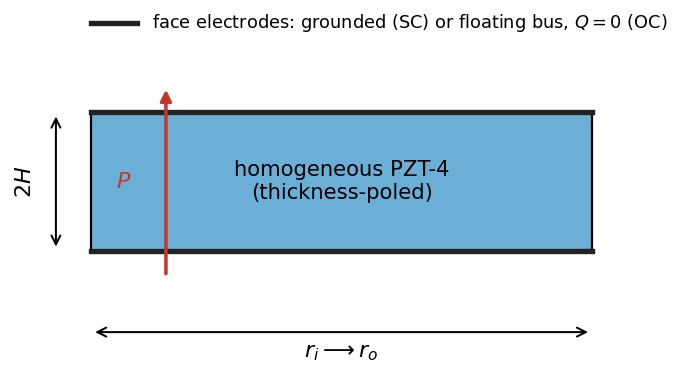
\includegraphics[width=0.75\linewidth]{piezo_p5_geometry.png}
\caption{Radial--thickness slice of the monolithic ring (not to scale).
One homogeneous, thickness-poled piezoceramic spans the full plate
thickness $2H$; both faces are electroded, grounded under short-circuit
or forming a single floating bus under open-circuit.}
\label{fig:geom}
\end{figure}

\subsection{Elastic-limit gate}\label{sec:elastic-gate}
At $(E,\nu)=(78.561\,\mathrm{GPa},\,0.28789)$ from \eqref{eq:Enu}, the
purely elastic free--free $n=0$ fundamental of the new mixed-edge
$4\times4$ agrees with an independently implemented closed-annulus
Kirchhoff solver \cite{mccune2026ring} to $4.8\times10^{-10}$ relative
(Supplementary~\S~S.2). This is the gate that must pass before any
coupled number below is trusted, and it uses none of the piezoelectric
code path.

\subsection{Short-circuit stiffening across four mechanical boundary
conditions}\label{sec:stiffening-results}
Table~\ref{tab:stiffening} reports the first $n=0$ flexural root of the
purely elastic ring and of the coupled short-circuit $6\times6$ (which,
by the theorem of \S\ref{sec:oc}, is simultaneously the open-circuit
root), on all four mechanical edge pairings. Short-circuit sits above
elastic at every pairing, as required by the sign of
\eqref{eq:stiffening}, and the split is a few percent rather than the
$10^{-3}$--$10^{-2}\,\%$ range found on the layered plate's own
short-circuit channel \cite{mccune2026piezo}: with no elastic host to
carry most of the bending stiffness, the piezoelectric coupling is no
longer a small correction to an otherwise elastic plate. The
clamped--free and free--clamped rows show that the split is not a
property of the free--free geometry alone, and that it is sensitive to
which edge is free: at this radius ratio the inner edge dominates
bending stiffness far more than the outer edge does (the clamped--free
elastic fundamental sits $90.4\%$ of the way from the free--free
fundamental to the clamped--clamped fundamental, while free--clamped
sits only $7.5\%$ of the way there), a finding specific to this
$r_i/r_o$ and reported as such, not as a universal ranking of edges.
Figure~\ref{fig:bc} shows the same four splits as a bar chart.

\begin{table}[H]
\centering
\caption{First $n=0$ flexural frequency, purely elastic ring versus the
coupled short-circuit operator (which coincides with open-circuit,
\S\ref{sec:oc}), all four mechanical edge pairings, in
$\mathrm{rad\,s^{-1}}$ (Hz in parentheses). C--F is clamped inner, free
outer; F--C is the swap.}
\label{tab:stiffening}
\small
\begin{tabular}{@{}lccc@{}}
\toprule
edge & elastic & SC $=$ OC & split \\
\midrule
F--F & 462.398 (73.593) & 471.365 (75.020) & $+1.939\%$ \\
C--C & 1726.890 (274.843) & 1757.694 (279.746) & $+1.784\%$ \\
C--F & 1605.443 (255.514) & 1637.922 (260.683) & $+2.023\%$ \\
F--C & 556.884 (88.631) & 564.900 (89.907) & $+1.439\%$ \\
\bottomrule
\end{tabular}
\end{table}

\begin{figure}[ht]
\centering
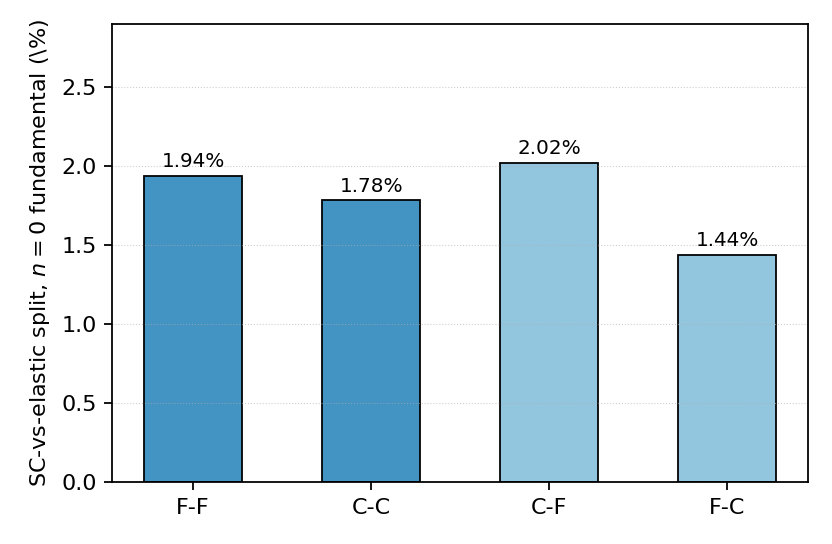
\includegraphics[width=0.6\linewidth]{piezo_p5_bc_stiffening.png}
\caption{Short-circuit-versus-elastic split of the $n=0$ fundamental,
Table~\ref{tab:stiffening}, by mechanical boundary condition.}
\label{fig:bc}
\end{figure}

The stiffening persists beyond the fundamental and beyond one thickness.
A sign-flip scan of the free--free channel up to
$6000\,\mathrm{rad\,s^{-1}}$ finds two further overtone pairs, both
still short-circuit above elastic ($+1.57\%$ and $+1.61\%$, against
$+1.94\%$ at the fundamental -- the split is not monotonic in overtone
index); the clamped--clamped channel shows the same pattern over one
further overtone ($+1.77\%$, against $+1.78\%$ at the fundamental). A
nine-point sweep of the ceramic thickness from $H/r_o=0.005$ to $0.18$,
at fixed radii, confirms a falsifiable prediction of the long-wave
reduction of \S\ref{sec:elastic} -- that the split is independent of
$H$ at leading order -- below $H/r_o\approx0.025$, where the split stays
flat near $1.94\%$; above that it drifts downward by about $4\%$
relative by $H/r_o=0.18$, a finite-thickness correction beyond the
long-wave leading order, consistent with Kirchhoff kinematics being
best justified in exactly the thin regime this paper's own geometry sits
in ($H/r_o\approx0.017$). Full numeric tables for both scans are in
Supplementary~\S~S.5.

\subsection{Finite-element cross-check}\label{sec:fe}
An independent coupled-field finite-element model (axisymmetric,
piezoelectric-plane elements, Lanczos eigensolver), built on the same
mesh, material block, and electrical-boundary conventions already
validated for the layered plate \cite{mccune2026piezo}, with the host
volume deleted and the piezoceramic volume filling the full thickness,
confirms both the coincidence theorem and the stiffening magnitude on
free--free $n=0$. The finite-element open-circuit and short-circuit
flexural modes agree with each other to five printed significant
figures -- the coincidence theorem is not only a Kirchhoff-theory
artifact, since the finite-element model carries genuinely
two-dimensional coupled-field kinematics -- and both sit $1.942\%$
above an uncoupled elastic control on the same mesh, against the
closed-form $+1.939\%$ of Table~\ref{tab:stiffening}: the
finite-element split reproduces the closed-form split to $0.1\%$ of its
value. This comparison is also what exposed the projection issue of
\S\ref{sec:sc}. The Gauss-law closure predicts $+2.347\%$ here, of which
finite elements recover only $83\%$, and $1/0.83\approx12/\pi^2$; the
same $12/\pi^2$ ratio separates that closure from a three-dimensional
finite-element model of a clamped piezoceramic annular sector
(Supplementary~\S~S.3). No spurious zero-frequency mode is present other
than the expected free--free rigid body, and the bending mode is
identified by the same through-thickness displacement discriminator used
throughout this series: transverse displacement of the same sign,
in-plane displacement of opposite sign, at the two faces at the outer
radius. A companion extensional mode on the same mesh does split between
open- and short-circuit ($+1.80\%$) -- confirming, as a disclosed side
observation and not a Paper~5 result, that the linear (membrane) field
does couple to extension even though it does not couple to bending, the
negative control anticipated in \S\ref{sec:kinematics}. Full provenance
is in Supplementary~\S~S.3.

\subsection{$e_{31}$ inverse from short-circuit-versus-elastic
frequency}\label{sec:inverse}
With $\cbar$ (equivalently $E,\nu$ through \eqref{eq:Enu}) held at its
known value, $e_{31}$ is the sole unknown, recovered by the same
residual-bisection and on-branch sensitivity recipe used throughout this
series \cite{mccune2026ring,mccune2026piezo}: a target frequency at the
true $e_{31}$ is bisected for, on a bracket containing a genuine sign
flip, with a wrong-sign bracket and an $e_{31}=0$ singular-limit check as
negative controls. Round-trip recovery of the injected $e_{31}$ from its
own forward frequency is exact to $2.5\times10^{-10}$ relative (bar
$10^{-6}$) on both the free--free and clamped--clamped channels; the
inverse machinery is not the issue, and the scientific content is the
propagated uncertainty. On-branch sensitivity gives
$\mathrm d\omega/\mathrm de_{31}=-3.618\,\mathrm{rad\,s^{-1}}$ per
$\mathrm{C\,m^{-2}}$ (free--free) and $-12.590$ (clamped--clamped);
propagating a $0.01\%$ relative frequency uncertainty through those
sensitivities gives $0.32\%$ and $0.34\%$ of $e_{31}$, respectively,
two orders of magnitude better conditioned than the short-circuit
inverse reported for the layered plate at a comparable thickness ratio
\cite{mccune2026piezo}, and roughly the same class as that paper's own
\emph{open}-circuit inverse -- because on this stacking the short-circuit
frequency already carries the full interior-profile coupling that, on the
layered plate, only the open-circuit channel could access. Do not invert
an open-circuit-versus-short-circuit split for $e_{31}$ here: no such
split exists (\S\ref{sec:oc}), and this single-observable inverse does
not jointly fit $\cbar$ and $e_{31}$ from one frequency.

One structural caveat applies to this inverse and is proved, not only
observed: the closing cubic of \S\ref{sec:sc} is invariant, as a set of
determinant rows up to an overall rescaling that does not move its
zeros, under the reflection $\eebar\to-\eebar$ composed with
$\chi\to-\chi$ (Supplementary~\S~S.4). Consequently every recovered root
$e_{31}$ has a bit-identical-frequency reflection twin,
$e_{31}^{\mathrm{twin}}=2(c_{13}^E/c_{33}^E)e_{33}-e_{31}
\approx13.80\,\mathrm{C\,m^{-2}}$ at this material point, and the
inversion bracket used throughout ($[1.0,8.0]\,\mathrm{C\,m^{-2}}$) is
chosen specifically to exclude both the twin and the intermediate value
at which the cubic's leading coefficient vanishes. This is the same
caveat documented for the layered plate's own open-circuit inverse
\cite{mccune2026piezo}, now derived explicitly for this operator rather
than carried over by analogy alone.

\section{Sensing admittance}\label{sec:Y}
\subsection{Voltage-driven admittance is a trivial capacitor}
\label{sec:Y-trivial}
Driving the plate electrically -- imposing a bus voltage $V$ rather than
solving $Q=0$ for it -- is the natural next step after \S\ref{sec:oc},
because it is exactly this construction that produced the layered
plate's identifying resonance/antiresonance pair. On this stacking it is
algebraically trivial rather than informative. The moment the driven
voltage produces is identically zero for every mechanical boundary
condition (\S\ref{sec:kinematics}), so the driven mechanical response is
identically zero at every frequency that is not itself a short-circuit
eigenfrequency, and the electrode charge is $Q=C_0V$ exactly, with no
motional correction at all. The undamped admittance is therefore
\begin{equation}
Y(\omega)=j\omega C_0
\label{eq:Ytrivial}
\end{equation}
for all $\omega$, a frequency-independent clamped capacitor, and
$k_{\mathrm{eff}}^2\equiv0$ for the flexural mode of this configuration
-- not a computational near-zero, an algebraic identity that holds for
any $\cbar$, $\eebar$, $\Xibar$, or geometry on this stacking. This is
the direct corollary of the coincidence theorem of \S\ref{sec:oc}: a
resonance/antiresonance pair requires a pole and a zero at two different
frequencies, and the theorem places both at the same frequency. It is
the textbook reason real bending-mode piezoelectric actuators and
sensors are built as unimorphs or bimorphs and not as symmetric
monolithic slabs, stated here as an exact, closed-form consequence of the
radial-determinant operator rather than assumed from general
electroacoustic reasoning.

\subsection{Force-driven sensing admittance}\label{sec:Y-sense}
Reading the same electromechanical coupling from its other port --
mechanical force in, electrical charge out -- is well posed, and it is
not trivial. A harmonic radial ring force $F$ at $r=r_F$ on the
still-grounded, still fully electroded short-circuit free--free plate
drives the two-region twelve-unknown system of \S\ref{sec:method}. Its
homogeneous kernel is confirmed to sit exactly at the already-validated
free--free short-circuit root: the driven system's own determinant and
the free-vibration determinant agree to machine precision at the F--F
fundamental of Table~\ref{tab:stiffening}. A global force-balance
identity, $2\pi\int_{r_i}^{r_o}r\,w(r)\,\mathrm dr=-F/(A_2\omega^2)$,
which must hold on both the purely elastic and the piezoelectrically
coupled version of this driven system at every off-resonance frequency,
confirms the sign of the one inhomogeneous interface row (the shear
jump) to $10^{-61}$ relative -- a check on the algebra, not a physical
prediction, but one that rules out the single most consequential class
of implementation error (a flipped sign on the load) independently of
any charge computation.

The electrode charge integrated over the \emph{entire} grounded face is,
however, identically zero at every driven frequency, by exactly the same
cancellation that produces \eqref{eq:Ytrivial}, read reciprocally: the
piezoelectric and dielectric contributions to the through-thickness
electric displacement at the face cancel pointwise once the governing
electrical equation is substituted in, leaving only an in-plane dielectric
flux that the insulated-rim electrical boundary condition forces to
integrate to zero over the whole face. A full-face sensing admittance
would therefore be a second trivial capacitor under a different name.
The nontrivial, resonance-showing output is the charge collected on a
proper subset of the grounded face -- a segmented electrode, both
segments still shorted to ground, current read from one segment. For an
inner partition $[r_i,r_*]$ of the face, the collected charge reduces to
the radial dielectric flux at the partition cut (Gauss's law through
the thickness applied to the leading-order field, which gives the face
charge as $\Xi_{11}\nabla^2\bar\phi\int_0^H(1-z^2/H^2)\,\mathrm dz$),
\begin{equation}
Q_{\mathrm{in}}(r_*;\omega)=\tfrac{4\pi}{3}H\Xi_{11}\,r_*\,\bar\phi'(r_*;\omega),
\qquad
Y_{\mathrm{sense}}[r_*](\omega):=\frac{Q_{\mathrm{in}}(r_*;\omega)}{F}.
\label{eq:Ysense}
\end{equation}
At the geometry of \S\ref{sec:forward} with $r_F=0.35\,\mathrm{m}$ and a
partition radius $r_*=0.30\,\mathrm{m}$ (chosen away from $r_F$ so a
load/cut coincidence is not built in), $Y_{\mathrm{sense}}$ is small and
smoothly varying away from resonance and grows by roughly four orders of
magnitude, with a clean sign change, within $0.01\,\mathrm{rad\,s^{-1}}$
of the free--free short-circuit fundamental of Table~\ref{tab:stiffening}
(Figure~\ref{fig:ysense}); no damping is present in this operator, so the
undamped magnitude formally diverges at the pole itself and the reported
sweep is a sign-change/blow-up diagnostic rather than a finite peak
height. As a limiting check, scaling $\eebar$ toward zero -- taking care
to scale the raw material constants $e_{31}$ and $e_{33}$ together, since
$\eebar$ itself is dominated by their combination at this material point
and does not approach zero if only $e_{31}$ is scaled -- drives
$Q_{\mathrm{in}}$ to zero linearly, matching the mechanical Helmholtz
branches to the purely elastic wavenumber over several orders of
magnitude in the scaling parameter (Supplementary~\S~S.7).

\begin{figure}[ht]
\centering
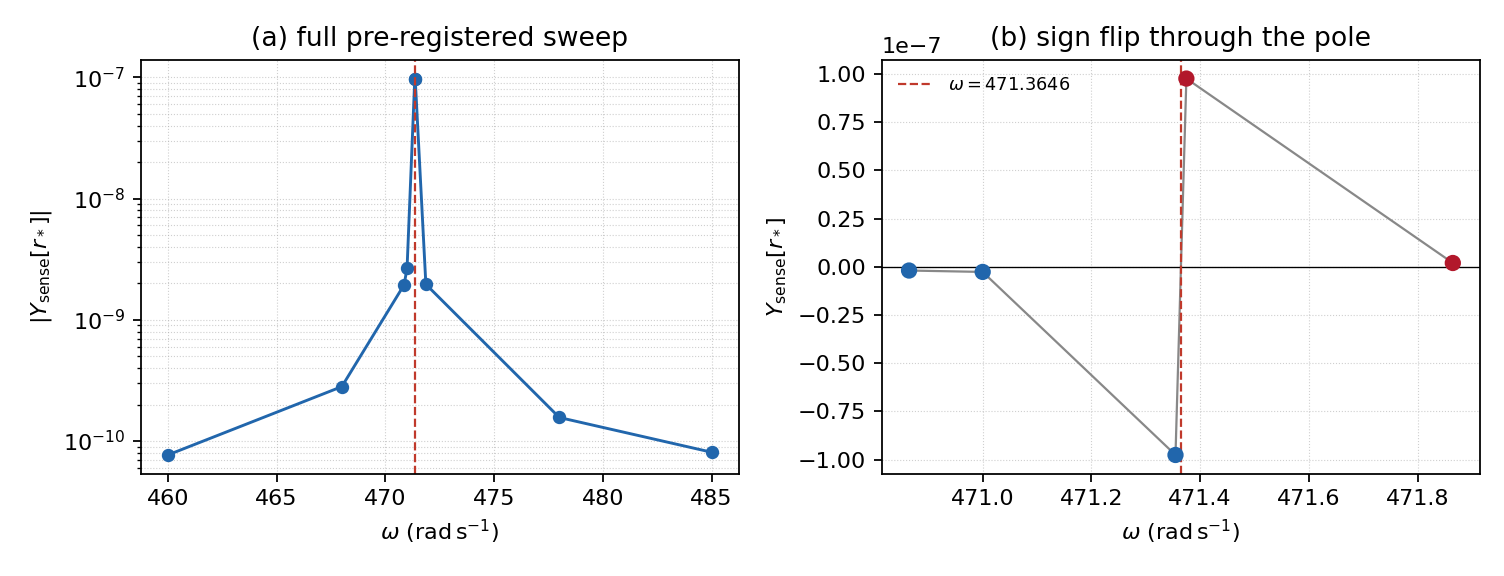
\includegraphics[width=0.92\linewidth]{piezo_p5_ysense_sweep.png}
\caption{Segmented-electrode sensing admittance $Y_{\mathrm{sense}}[r_*]$
near the free--free short-circuit fundamental
($471.3646\,\mathrm{rad\,s^{-1}}$), $r_F=0.35\,\mathrm m$,
$r_*=0.30\,\mathrm m$. (a) magnitude across the pre-registered validation
sweep; (b) sign flip through the pole, undamped. Not a dense resonance
curve -- the nine points are the pre-registered validation gate, not a
fitted or interpolated response.}
\label{fig:ysense}
\end{figure}

The applied reading is the one worth stating plainly: this specimen
cannot be voltage-actuated in flexure, and it cannot be sensed in flexure
from a single full-face electrode either -- both are exact zeros of the
same underlying theorem -- but it \emph{can} be sensed, with a genuine
resonant response, from a segmented electrode reading the mechanical
side of the coupling. For a transducer engineer working with a
symmetric, thickness-poled monolithic stack, that is an actionable design
implication, not only a pair of null results: actuation on this specimen
belongs on the extensional (contour) side of the same electromechanical
coupling, disclosed in \S\ref{sec:fe} and left as claim~C of this series
\cite{mccune2026piezo}, while sensing of the flexural mode itself
requires partitioning the electrode rather than adding instrumentation
elsewhere.

\section{Discussion}\label{sec:disc}
The layered and monolithic papers of this series now bracket the same
electromechanical question from opposite stackings, using the same
material, the same exact radial-determinant method, and the same
inverse-recovery recipe. Offsetting a thin piezoceramic layer from a
plate's neutral axis, as in the layered construction, makes a uniform
electrode voltage a flexural actuator and turns the free--free
open-circuit-versus-short-circuit split into the identifying observable
for $e_{31}$; the short-circuit channel alone is nearly useless there,
propagating $0.01\%$ frequency precision to hundreds of percent of
$e_{31}$ \cite{mccune2026piezo}. Removing the host and centering the same
ceramic on the neutral axis, as here, removes that actuation mechanism
entirely -- not approximately, but as an algebraic identity holding for
every mechanical boundary condition -- and simultaneously turns the
short-circuit channel itself into a well-conditioned observable, because
the whole plate thickness is now piezoceramic rather than a thin
fraction of it. Neither result is more fundamental than the other; they
are the same electromechanical coupling read through two different
mechanical constructions of the same material system, and a reader
choosing between a layered sandwich and a monolithic ring for a real
identification task should expect exactly this trade: the layered plate
needs an open-circuit measurement and a rank-1 correction to identify
$e_{31}$ at all, while the monolithic ring identifies it directly from
short-circuit flexure but loses the electrode-voltage resonance/
antiresonance method as a sensing route.

Limits, so they are not rediscovered as objections. No literature
frequency table exists for a homogeneous, thickness-poled, Kirchhoff-%
class piezoceramic annulus at the time of writing; the external check
here is finite-element, the same role finite elements played for the
layered plate's own open-circuit split \cite{mccune2026piezo}, and it
confirms both the coincidence theorem and the stiffening magnitude with
genuinely two-dimensional coupled-field kinematics, not only within
Kirchhoff theory. The coincidence theorem and the trivial voltage-driven
admittance are properties of this ansatz -- fully electroded faces,
insulated rims -- and do not extend to a plate with a partially covered
or patterned electrode, which is a different electrical boundary
condition and not addressed here beyond the sensing partition of
\S\ref{sec:Y-sense}. The force-driven sensing construction is axisymmetric
and free--free only; clamped and mixed-edge sensing variants are the same
interface-row substitution used for the free-vibration mixed-edge
determinants and are left for later work. In-plane (extensional, contour)
piezoelectric coupling on this same monolithic stacking is disclosed as a
genuine effect in \S\ref{sec:fe} but is not built here; it is claim~C of
this series \cite{mccune2026piezo} and a natural companion paper on the
same physical hardware, since an impedance-analyzer measurement of a real
specimen would see exactly that contour response, not the flexural one
studied here. A radially poled, shear-actuated specimen on Mindlin
kinematics \cite{parashar2013} is a different poling axis, a different
actuation mechanism, and a different plate theory, and is not scored by
this Kirchhoff monolithic operator. No physical specimen is reported
here; were one tested, short-circuit flexure of Table~\ref{tab:stiffening}
is the observable for $e_{31}$, and a segmented-electrode measurement of
$Y_{\mathrm{sense}}$ under mechanical excitation, not an impedance-%
analyzer voltage sweep, is the observable for sensing.

The elastic ring and the layered piezoelectric plate of this series
\cite{mccune2026ring,mccune2026piezo} are the baselines this construction
sits on. The present frequencies do not re-score either paper's
literature tables; they extend the same exact method to a stacking
neither paper addressed, and report both a coincidence theorem and a
sensing alternative that the layered plate's own geometry does not
require.

\section{Conclusions}\label{sec:conc}
A homogeneous, thickness-polarized piezoceramic ring, electroded only on
its two faces, has an exact short-circuit $6\times6$ radial-determinant
solver in the same Helmholtz/Bessel family as the corresponding layered
piezoelectric plate, whose elastic limit agrees with an independent
closed-ring solver to $4.8\times10^{-10}$ relative. Because a spatially
uniform electrode voltage produces a through-thickness field that is
symmetric about this plate's own neutral surface, its piezoelectric
moment integrates to exactly zero: fully electroded open-circuit flexure
coincides with short-circuit flexure for every mechanical boundary
condition tested, not only the special case that held on the layered
plate, and the voltage-driven admittance is a frequency-independent
capacitor with $k_{\mathrm{eff}}^2\equiv0$. Finite elements confirm both
the coincidence, to five significant figures, and the stiffening
magnitude, reproducing the closed-form split to $0.1\%$ of its value with
genuinely two-dimensional coupled-field kinematics, once the electrical
equation is projected consistently with the mechanical one. The
piezoelectric signal on this stacking is therefore the
short-circuit-versus-elastic frequency gap itself: $+1.94\%$,
$+1.78\%$, $+2.02\%$, and $+1.44\%$ on the free--free,
clamped--clamped, clamped--free, and free--clamped $n=0$ fundamentals of
a representative PZT-4 geometry, propagating a $0.01\%$ frequency
uncertainty to $0.32$--$0.34\%$ of $e_{31}$ -- two orders of
magnitude better conditioned than the corresponding short-circuit inverse
on a layered sandwich of the same material. Because the electrode-voltage
route to sensing is closed off by the same theorem that closes off
actuation, sensing is read from the mechanical side instead: a harmonic
radial force drives a genuinely resonant charge response on a segmented
electrode, even though the same force drives an identically zero charge
on the full electroded face. A symmetric, thickness-poled monolithic
plate can be neither voltage-actuated nor full-electrode-sensed in
flexure, but it can be force-driven and segment-sensed -- the textbook
justification for unimorph and bimorph bending actuators, derived here as
an exact property of the radial-determinant operator with a working
sensing alternative rather than only a limitation.

\section*{Data and code availability}
The solver implementing the operators of this paper, and the scripts
that produced every number and table here, extend the public tree
accompanying \cite{mccune2026ring}.

\section*{Funding}
This research did not receive any specific grant from funding agencies in the
public, commercial, or not-for-profit sectors.

\section*{Acknowledgments}
The computation for this work was performed on The Mill HPC cluster at
Missouri University of Science and Technology \cite{mill2024}. GPU resources
were not used.

\section*{CRediT authorship contribution statement}
\textbf{Garrek McCune:} Conceptualization, Methodology, Software, Validation,
Formal analysis, Investigation, Writing -- original draft, Writing -- review \&
editing, Visualization. \textbf{Daniel Stutts:} Conceptualization,
Supervision.

\section*{Declaration of generative AI and AI-assisted technologies}
During the preparation of this work, the authors used generative AI tools to
assist with manuscript and code organization, drafting, editing, and
formatting. After using these tools, the authors reviewed and edited the
content as needed and take full responsibility for the content of this
publication.
\normalsize

\clearpage
\begin{thebibliography}{99}\small
\setlength{\itemsep}{0pt}
\setlength{\parsep}{0pt}
\bibitem{seok1} J. Seok, H.F. Tiersten, ``Free vibrations of annular sector
cantilever plates. Part 1: out-of-plane motion,'' J. Sound Vib. 271 (2004)
757--772. \url{https://doi.org/10.1016/S0022-460X(03)00414-0}.
\bibitem{seok2} J. Seok, H.F. Tiersten, ``Free vibrations of annular sector
cantilever plates. Part 2: in-plane motion,'' J. Sound Vib. 271 (2004)
773--787. \url{https://doi.org/10.1016/S0022-460X(03)00415-2}.
\bibitem{duan2005} W.H. Duan, S.T. Quek, Q. Wang, ``Free vibration analysis
of piezoelectric coupled thin and thick annular plate,'' J. Sound Vib. 281
(2005) 119--139. \url{https://doi.org/10.1016/j.jsv.2004.01.005}.
\bibitem{liu2002} X. Liu, Q. Wang, S.T. Quek, ``Analytical solution for free
vibration of piezoelectric coupled moderately thick circular plates,''
Int. J. Solids Struct. 39 (2002) 2129--2151.
\url{https://doi.org/10.1016/S0020-7683(02)00079-3}.
\bibitem{tiersten1969} H.F. Tiersten, \emph{Linear Piezoelectric Plate
Vibrations}, Plenum Press, New York, 1969.
\bibitem{holland1966} R. Holland, ``Numerical studies of elastic-disk
contour modes lacking axial symmetry,'' J. Acoust. Soc. Am. 40 (1966)
1051--1057. \url{https://doi.org/10.1121/1.1910187}.
\bibitem{ieee176} IEEE, \emph{IEEE Standard on Piezoelectricity}, ANSI/IEEE
Std 176-1987, IEEE, New York (1988).
\bibitem{parashar2013} S.K. Parashar, ``Modeling and analysis of
shear-induced flexural vibrations of annular piezoceramic actuators,''
J. Intell. Mater. Syst. Struct. 24 (2013).
\url{https://doi.org/10.1177/1045389X13478273}.
\bibitem{mccune2026ring} G. McCune, D. Stutts, ``Exact radial-determinant
frequencies of annular and circular plates: the closed-ring and solid-disk
limits of the sector wave-function method,'' submitted (2026).
\bibitem{mccune2026piezo} G. McCune, D. Stutts, ``Exact radial-determinant
frequencies of a piezoelectric annular plate, and inverse recovery of
$e_{31}$ from open-circuit flexure,'' submitted (2026).
\bibitem{ansys} ANSYS, Inc., \emph{ANSYS Mechanical APDL}, Release 2025 R1,
ANSYS, Inc., Canonsburg, PA, USA (2025). Used for finite-element validation
only.
\bibitem{mill2024} Missouri University of Science and Technology, ``The Mill
HPC Cluster,'' \emph{The Mill} (2024), Article 1.
\url{https://scholarsmine.mst.edu/the-mill/1},
\url{https://doi.org/10.71674/PH64-N397}.
\end{thebibliography}
\end{document}
